% Graphic for TeX using PGF
% Title: /Users/ziqiaozhou/sclockgit/ccs16/fig/page_fault.dia
% Creator: Dia v0.97.2
% CreationDate: Wed Aug 10 17:23:04 2016
% For: ziqiaozhou
% \usepackage{tikz}
% The following commands are not supported in PSTricks at present
% We define them conditionally, so when they are implemented,
% this pgf file will use them.
\ifx\du\undefined
  \newlength{\du}
\fi
\setlength{\du}{15\unitlength}
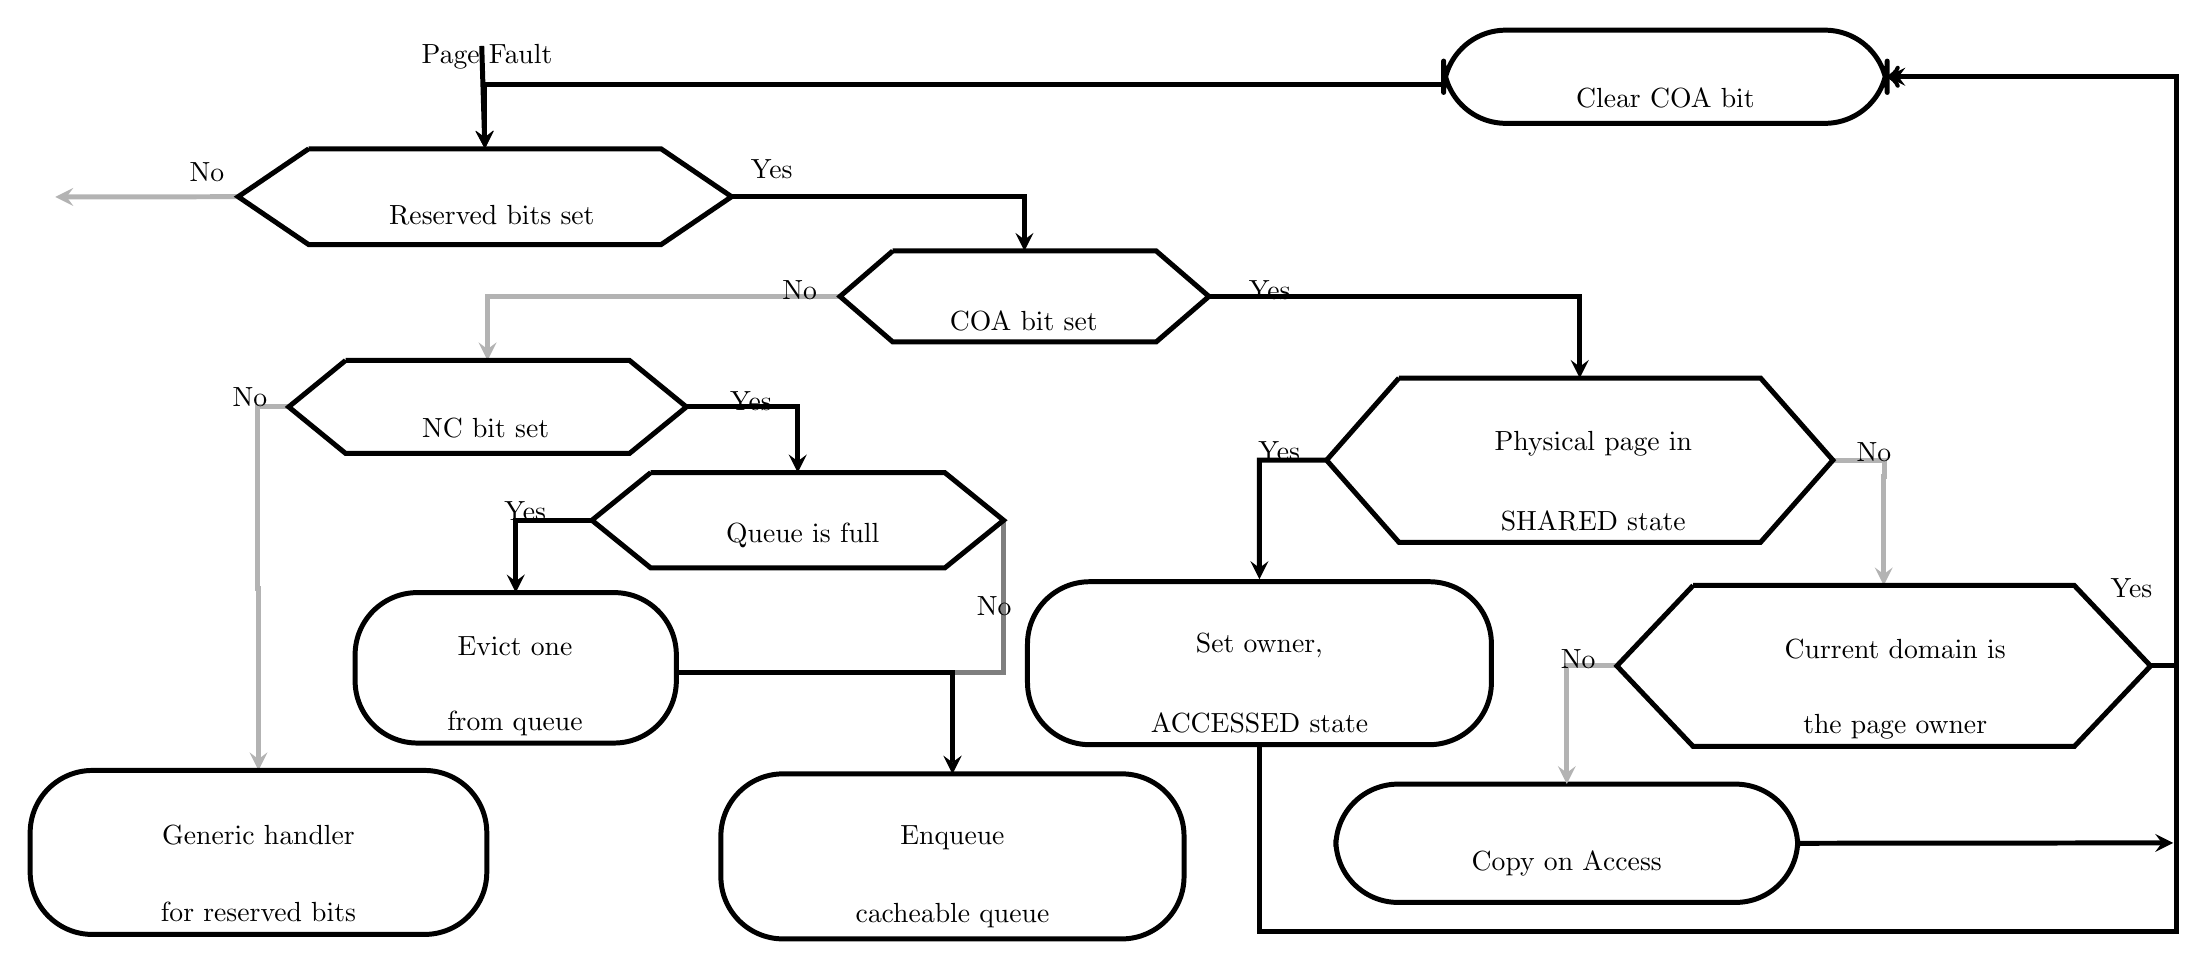
\begin{tikzpicture}
\pgftransformxscale{1.000000}
\pgftransformyscale{-1.000000}
\definecolor{dialinecolor}{rgb}{0.000000, 0.000000, 0.000000}
\pgfsetstrokecolor{dialinecolor}
\definecolor{dialinecolor}{rgb}{1.000000, 1.000000, 1.000000}
\pgfsetfillcolor{dialinecolor}
\pgfsetlinewidth{0.120000\du}
\pgfsetdash{}{0pt}
\pgfsetdash{}{0pt}
\pgfsetroundjoin
{\pgfsetcornersarced{\pgfpoint{1.500000\du}{1.500000\du}}\definecolor{dialinecolor}{rgb}{1.000000, 1.000000, 1.000000}
\pgfsetfillcolor{dialinecolor}
\fill (44.178700\du,40.885800\du)--(44.178700\du,43.736246\du)--(55.304441\du,43.736246\du)--(55.304441\du,40.885800\du)--cycle;
}{\pgfsetcornersarced{\pgfpoint{1.500000\du}{1.500000\du}}\definecolor{dialinecolor}{rgb}{0.000000, 0.000000, 0.000000}
\pgfsetstrokecolor{dialinecolor}
\draw (44.178700\du,40.885800\du)--(44.178700\du,43.736246\du)--(55.304441\du,43.736246\du)--(55.304441\du,40.885800\du)--cycle;
}% setfont left to latex
\definecolor{dialinecolor}{rgb}{0.000000, 0.000000, 0.000000}
\pgfsetstrokecolor{dialinecolor}
\node at (49.741600\du,42.816100\du){Copy on Access};
\pgfsetlinewidth{0.120000\du}
\pgfsetdash{}{0pt}
\pgfsetdash{}{0pt}
\pgfsetmiterjoin
\pgfsetbuttcap
{
\definecolor{dialinecolor}{rgb}{0.000000, 0.000000, 0.000000}
\pgfsetfillcolor{dialinecolor}
% was here!!!
\pgfsetarrowsend{stealth}
{\pgfsetcornersarced{\pgfpoint{0.000000\du}{0.000000\du}}\definecolor{dialinecolor}{rgb}{0.000000, 0.000000, 0.000000}
\pgfsetstrokecolor{dialinecolor}
\draw (41.120700\du,29.137700\du)--(50.053500\du,29.137700\du)--(50.053500\du,31.104500\du);
}}
\pgfsetlinewidth{0.120000\du}
\pgfsetdash{}{0pt}
\pgfsetdash{}{0pt}
\pgfsetmiterjoin
\pgfsetbuttcap
{
\definecolor{dialinecolor}{rgb}{0.701961, 0.701961, 0.701961}
\pgfsetfillcolor{dialinecolor}
% was here!!!
\pgfsetarrowsend{stealth}
{\pgfsetcornersarced{\pgfpoint{0.000000\du}{0.000000\du}}\definecolor{dialinecolor}{rgb}{0.701961, 0.701961, 0.701961}
\pgfsetstrokecolor{dialinecolor}
\draw (32.233300\du,29.137661\du)--(23.742899\du,29.137661\du)--(23.742899\du,30.680600\du);
}}
\pgfsetlinewidth{0.120000\du}
\pgfsetdash{}{0pt}
\pgfsetdash{}{0pt}
\pgfsetmiterjoin
\pgfsetbuttcap
{
\definecolor{dialinecolor}{rgb}{0.701961, 0.701961, 0.701961}
\pgfsetfillcolor{dialinecolor}
% was here!!!
\pgfsetarrowsend{stealth}
{\pgfsetcornersarced{\pgfpoint{0.000000\du}{0.000000\du}}\definecolor{dialinecolor}{rgb}{0.701961, 0.701961, 0.701961}
\pgfsetstrokecolor{dialinecolor}
\draw (18.952800\du,31.799200\du)--(18.208500\du,31.799200\du)--(18.208500\du,36.173400\du)--(18.224400\du,36.173400\du)--(18.224400\du,40.556500\du);
}}
\pgfsetlinewidth{0.120000\du}
\pgfsetdash{}{0pt}
\pgfsetdash{}{0pt}
\pgfsetmiterjoin
\pgfsetbuttcap
{
\definecolor{dialinecolor}{rgb}{0.000000, 0.000000, 0.000000}
\pgfsetfillcolor{dialinecolor}
% was here!!!
\pgfsetarrowsend{stealth}
{\pgfsetcornersarced{\pgfpoint{0.000000\du}{0.000000\du}}\definecolor{dialinecolor}{rgb}{0.000000, 0.000000, 0.000000}
\pgfsetstrokecolor{dialinecolor}
\draw (26.256500\du,34.529646\du)--(24.421112\du,34.529646\du)--(24.421112\du,36.272100\du);
}}
\pgfsetlinewidth{0.120000\du}
\pgfsetdash{}{0pt}
\pgfsetdash{}{0pt}
\pgfsetroundjoin
{\pgfsetcornersarced{\pgfpoint{1.500000\du}{1.500000\du}}\definecolor{dialinecolor}{rgb}{1.000000, 1.000000, 1.000000}
\pgfsetfillcolor{dialinecolor}
\fill (12.724400\du,40.556500\du)--(12.724400\du,44.507214\du)--(23.724404\du,44.507214\du)--(23.724404\du,40.556500\du)--cycle;
}{\pgfsetcornersarced{\pgfpoint{1.500000\du}{1.500000\du}}\definecolor{dialinecolor}{rgb}{0.000000, 0.000000, 0.000000}
\pgfsetstrokecolor{dialinecolor}
\draw (12.724400\du,40.556500\du)--(12.724400\du,44.507214\du)--(23.724404\du,44.507214\du)--(23.724404\du,40.556500\du)--cycle;
}% setfont left to latex
\definecolor{dialinecolor}{rgb}{0.000000, 0.000000, 0.000000}
\pgfsetstrokecolor{dialinecolor}
\node at (18.224400\du,42.101939\du){Generic handler };
% setfont left to latex
\definecolor{dialinecolor}{rgb}{0.000000, 0.000000, 0.000000}
\pgfsetstrokecolor{dialinecolor}
\node at (18.224400\du,43.971661\du){for reserved bits};
% setfont left to latex
\definecolor{dialinecolor}{rgb}{0.000000, 0.000000, 0.000000}
\pgfsetstrokecolor{dialinecolor}
\node[anchor=west] at (33.445900\du,32.388100\du){};
\pgfsetlinewidth{0.120000\du}
\pgfsetdash{}{0pt}
\pgfsetdash{}{0pt}
\pgfsetmiterjoin
\pgfsetbuttcap
{
\definecolor{dialinecolor}{rgb}{0.000000, 0.000000, 0.000000}
\pgfsetfillcolor{dialinecolor}
% was here!!!
\pgfsetarrowsend{stealth}
{\pgfsetcornersarced{\pgfpoint{0.000000\du}{0.000000\du}}\definecolor{dialinecolor}{rgb}{0.000000, 0.000000, 0.000000}
\pgfsetstrokecolor{dialinecolor}
\draw (43.954600\du,33.082200\du)--(42.337565\du,33.082200\du)--(42.337550\du,35.949681\du);
}}
\pgfsetlinewidth{0.120000\du}
\pgfsetdash{}{0pt}
\pgfsetdash{}{0pt}
\pgfsetbuttcap
{
\definecolor{dialinecolor}{rgb}{0.000000, 0.000000, 0.000000}
\pgfsetfillcolor{dialinecolor}
% was here!!!
\pgfsetarrowsend{stealth}
\definecolor{dialinecolor}{rgb}{0.000000, 0.000000, 0.000000}
\pgfsetstrokecolor{dialinecolor}
\draw (55.304500\du,42.311100\du)--(64.350700\du,42.301600\du);
}
\pgfsetlinewidth{0.120000\du}
\pgfsetdash{}{0pt}
\pgfsetdash{}{0pt}
\pgfsetmiterjoin
\pgfsetbuttcap
{
\definecolor{dialinecolor}{rgb}{0.701961, 0.701961, 0.701961}
\pgfsetfillcolor{dialinecolor}
% was here!!!
\pgfsetarrowsend{stealth}
{\pgfsetcornersarced{\pgfpoint{0.000000\du}{0.000000\du}}\definecolor{dialinecolor}{rgb}{0.701961, 0.701961, 0.701961}
\pgfsetstrokecolor{dialinecolor}
\draw (56.152400\du,33.082200\du)--(57.388800\du,33.082200\du)--(57.388800\du,33.479100\du)--(57.376400\du,33.479100\du)--(57.376400\du,36.100900\du);
}}
\pgfsetlinewidth{0.120000\du}
\pgfsetdash{}{0pt}
\pgfsetdash{}{0pt}
\pgfsetroundjoin
{\pgfsetcornersarced{\pgfpoint{1.500000\du}{1.500000\du}}\definecolor{dialinecolor}{rgb}{1.000000, 1.000000, 1.000000}
\pgfsetfillcolor{dialinecolor}
\fill (46.773500\du,22.723600\du)--(46.773500\du,24.967720\du)--(57.460014\du,24.967720\du)--(57.460014\du,22.723600\du)--cycle;
}{\pgfsetcornersarced{\pgfpoint{1.500000\du}{1.500000\du}}\definecolor{dialinecolor}{rgb}{0.000000, 0.000000, 0.000000}
\pgfsetstrokecolor{dialinecolor}
\draw (46.773500\du,22.723600\du)--(46.773500\du,24.967720\du)--(57.460014\du,24.967720\du)--(57.460014\du,22.723600\du)--cycle;
}% setfont left to latex
\definecolor{dialinecolor}{rgb}{0.000000, 0.000000, 0.000000}
\pgfsetstrokecolor{dialinecolor}
\node at (52.116700\du,24.350700\du){Clear COA bit};
% setfont left to latex
\definecolor{dialinecolor}{rgb}{0.000000, 0.000000, 0.000000}
\pgfsetstrokecolor{dialinecolor}
\node[anchor=west] at (52.116700\du,24.350700\du){};
\pgfsetlinewidth{0.120000\du}
\pgfsetdash{}{0pt}
\pgfsetdash{}{0pt}
\pgfsetmiterjoin
\pgfsetbuttcap
{
\definecolor{dialinecolor}{rgb}{0.000000, 0.000000, 0.000000}
\pgfsetfillcolor{dialinecolor}
% was here!!!
\pgfsetarrowsend{stealth}
{\pgfsetcornersarced{\pgfpoint{0.000000\du}{0.000000\du}}\definecolor{dialinecolor}{rgb}{0.000000, 0.000000, 0.000000}
\pgfsetstrokecolor{dialinecolor}
\draw (46.773500\du,23.845700\du)--(46.773500\du,24.025800\du)--(23.678300\du,24.025800\du)--(23.678300\du,25.581500\du);
}}
\pgfsetlinewidth{0.120000\du}
\pgfsetdash{}{0pt}
\pgfsetdash{}{0pt}
\pgfsetmiterjoin
\pgfsetbuttcap
{
\definecolor{dialinecolor}{rgb}{0.498039, 0.498039, 0.498039}
\pgfsetfillcolor{dialinecolor}
% was here!!!
\pgfsetarrowsend{stealth}
{\pgfsetcornersarced{\pgfpoint{0.000000\du}{0.000000\du}}\definecolor{dialinecolor}{rgb}{0.498039, 0.498039, 0.498039}
\pgfsetstrokecolor{dialinecolor}
\draw (36.174500\du,34.529600\du)--(36.174500\du,38.203600\du)--(34.942100\du,38.203600\du)--(34.942100\du,40.638400\du);
}}
\pgfsetlinewidth{0.120000\du}
\pgfsetdash{}{0pt}
\pgfsetdash{}{0pt}
\pgfsetmiterjoin
\pgfsetbuttcap
{
\definecolor{dialinecolor}{rgb}{0.000000, 0.000000, 0.000000}
\pgfsetfillcolor{dialinecolor}
% was here!!!
\pgfsetarrowsend{stealth}
{\pgfsetcornersarced{\pgfpoint{0.000000\du}{0.000000\du}}\definecolor{dialinecolor}{rgb}{0.000000, 0.000000, 0.000000}
\pgfsetstrokecolor{dialinecolor}
\draw (28.290300\du,38.084300\du)--(28.290300\du,38.203600\du)--(34.942100\du,38.203600\du)--(34.942100\du,40.638400\du);
}}
\pgfsetlinewidth{0.120000\du}
\pgfsetdash{}{0pt}
\pgfsetdash{}{0pt}
\pgfsetmiterjoin
\pgfsetbuttcap
{
\definecolor{dialinecolor}{rgb}{0.000000, 0.000000, 0.000000}
\pgfsetfillcolor{dialinecolor}
% was here!!!
\pgfsetarrowsend{stealth}
{\pgfsetcornersarced{\pgfpoint{0.000000\du}{0.000000\du}}\definecolor{dialinecolor}{rgb}{0.000000, 0.000000, 0.000000}
\pgfsetstrokecolor{dialinecolor}
\draw (63.804400\du,38.039300\du)--(64.432500\du,38.039300\du)--(64.432500\du,23.845700\du)--(57.460000\du,23.845700\du);
}}
\pgfsetlinewidth{0.120000\du}
\pgfsetdash{}{0pt}
\pgfsetdash{}{0pt}
\pgfsetmiterjoin
\pgfsetbuttcap
{
\definecolor{dialinecolor}{rgb}{0.701961, 0.701961, 0.701961}
\pgfsetfillcolor{dialinecolor}
% was here!!!
\pgfsetarrowsend{stealth}
{\pgfsetcornersarced{\pgfpoint{0.000000\du}{0.000000\du}}\definecolor{dialinecolor}{rgb}{0.701961, 0.701961, 0.701961}
\pgfsetstrokecolor{dialinecolor}
\draw (50.948300\du,38.039309\du)--(49.741570\du,38.039309\du)--(49.741570\du,40.885800\du);
}}
\pgfsetlinewidth{0.120000\du}
\pgfsetdash{}{0pt}
\pgfsetdash{}{0pt}
\pgfsetmiterjoin
\pgfsetbuttcap
{
\definecolor{dialinecolor}{rgb}{0.000000, 0.000000, 0.000000}
\pgfsetfillcolor{dialinecolor}
% was here!!!
\pgfsetarrowsend{stealth}
{\pgfsetcornersarced{\pgfpoint{0.000000\du}{0.000000\du}}\definecolor{dialinecolor}{rgb}{0.000000, 0.000000, 0.000000}
\pgfsetstrokecolor{dialinecolor}
\draw (29.621318\du,26.735235\du)--(36.676990\du,26.735235\du)--(36.676990\du,28.042800\du);
}}
% setfont left to latex
\definecolor{dialinecolor}{rgb}{0.000000, 0.000000, 0.000000}
\pgfsetstrokecolor{dialinecolor}
\node at (23.728400\du,23.371077\du){Page Fault};
\pgfsetlinewidth{0.120000\du}
\pgfsetdash{}{0pt}
\pgfsetdash{}{0pt}
\pgfsetbuttcap
{
\definecolor{dialinecolor}{rgb}{0.000000, 0.000000, 0.000000}
\pgfsetfillcolor{dialinecolor}
% was here!!!
\pgfsetarrowsend{stealth}
\definecolor{dialinecolor}{rgb}{0.000000, 0.000000, 0.000000}
\pgfsetstrokecolor{dialinecolor}
\draw (23.602500\du,23.103800\du)--(23.678300\du,25.581500\du);
}
\pgfsetlinewidth{0.120000\du}
\pgfsetdash{}{0pt}
\pgfsetdash{}{0pt}
\pgfsetbuttcap
{
\definecolor{dialinecolor}{rgb}{0.701961, 0.701961, 0.701961}
\pgfsetfillcolor{dialinecolor}
% was here!!!
\pgfsetarrowsend{stealth}
\definecolor{dialinecolor}{rgb}{0.701961, 0.701961, 0.701961}
\pgfsetstrokecolor{dialinecolor}
\draw (17.735200\du,26.735200\du)--(13.329000\du,26.741200\du);
}
% setfont left to latex
\definecolor{dialinecolor}{rgb}{0.000000, 0.000000, 0.000000}
\pgfsetstrokecolor{dialinecolor}
\node at (42.587100\du,28.984200\du){Yes};
% setfont left to latex
\definecolor{dialinecolor}{rgb}{0.000000, 0.000000, 0.000000}
\pgfsetstrokecolor{dialinecolor}
\node at (31.259500\du,28.984200\du){No};
\pgfsetlinewidth{0.120000\du}
\pgfsetdash{}{0pt}
\pgfsetdash{}{0pt}
\pgfsetbuttcap
\pgfsetmiterjoin
\pgfsetlinewidth{0.120000\du}
\pgfsetbuttcap
\pgfsetmiterjoin
\pgfsetdash{}{0pt}
\definecolor{dialinecolor}{rgb}{1.000000, 1.000000, 1.000000}
\pgfsetfillcolor{dialinecolor}
\pgfpathmoveto{\pgfpoint{33.502926\du}{28.042800\du}}
\pgfpathlineto{\pgfpoint{39.851053\du}{28.042800\du}}
\pgfpathlineto{\pgfpoint{41.120679\du}{29.137661\du}}
\pgfpathlineto{\pgfpoint{39.851053\du}{30.232522\du}}
\pgfpathlineto{\pgfpoint{33.502926\du}{30.232522\du}}
\pgfpathlineto{\pgfpoint{32.233300\du}{29.137661\du}}
\pgfpathlineto{\pgfpoint{33.502926\du}{28.042800\du}}
\pgfusepath{fill}
\definecolor{dialinecolor}{rgb}{0.000000, 0.000000, 0.000000}
\pgfsetstrokecolor{dialinecolor}
\pgfpathmoveto{\pgfpoint{33.502926\du}{28.042800\du}}
\pgfpathlineto{\pgfpoint{39.851053\du}{28.042800\du}}
\pgfpathlineto{\pgfpoint{41.120679\du}{29.137661\du}}
\pgfpathlineto{\pgfpoint{39.851053\du}{30.232522\du}}
\pgfpathlineto{\pgfpoint{33.502926\du}{30.232522\du}}
\pgfpathlineto{\pgfpoint{32.233300\du}{29.137661\du}}
\pgfpathlineto{\pgfpoint{33.502926\du}{28.042800\du}}
\pgfusepath{stroke}
% setfont left to latex
\definecolor{dialinecolor}{rgb}{0.000000, 0.000000, 0.000000}
\pgfsetstrokecolor{dialinecolor}
\node at (36.676990\du,29.511606\du){};
% setfont left to latex
\definecolor{dialinecolor}{rgb}{0.000000, 0.000000, 0.000000}
\pgfsetstrokecolor{dialinecolor}
\node at (36.660300\du,29.723600\du){COA bit set};
% setfont left to latex
\definecolor{dialinecolor}{rgb}{0.000000, 0.000000, 0.000000}
\pgfsetstrokecolor{dialinecolor}
\node at (30.589200\du,26.078100\du){Yes};
\pgfsetlinewidth{0.120000\du}
\pgfsetdash{}{0pt}
\pgfsetdash{}{0pt}
\pgfsetbuttcap
\pgfsetmiterjoin
\pgfsetlinewidth{0.120000\du}
\pgfsetbuttcap
\pgfsetmiterjoin
\pgfsetdash{}{0pt}
\definecolor{dialinecolor}{rgb}{1.000000, 1.000000, 1.000000}
\pgfsetfillcolor{dialinecolor}
\pgfpathmoveto{\pgfpoint{19.433217\du}{25.581500\du}}
\pgfpathlineto{\pgfpoint{27.923301\du}{25.581500\du}}
\pgfpathlineto{\pgfpoint{29.621318\du}{26.735235\du}}
\pgfpathlineto{\pgfpoint{27.923301\du}{27.888970\du}}
\pgfpathlineto{\pgfpoint{19.433217\du}{27.888970\du}}
\pgfpathlineto{\pgfpoint{17.735200\du}{26.735235\du}}
\pgfpathlineto{\pgfpoint{19.433217\du}{25.581500\du}}
\pgfusepath{fill}
\definecolor{dialinecolor}{rgb}{0.000000, 0.000000, 0.000000}
\pgfsetstrokecolor{dialinecolor}
\pgfpathmoveto{\pgfpoint{19.433217\du}{25.581500\du}}
\pgfpathlineto{\pgfpoint{27.923301\du}{25.581500\du}}
\pgfpathlineto{\pgfpoint{29.621318\du}{26.735235\du}}
\pgfpathlineto{\pgfpoint{27.923301\du}{27.888970\du}}
\pgfpathlineto{\pgfpoint{19.433217\du}{27.888970\du}}
\pgfpathlineto{\pgfpoint{17.735200\du}{26.735235\du}}
\pgfpathlineto{\pgfpoint{19.433217\du}{25.581500\du}}
\pgfusepath{stroke}
% setfont left to latex
\definecolor{dialinecolor}{rgb}{0.000000, 0.000000, 0.000000}
\pgfsetstrokecolor{dialinecolor}
\node at (23.678259\du,27.109180\du){};
% setfont left to latex
\definecolor{dialinecolor}{rgb}{0.000000, 0.000000, 0.000000}
\pgfsetstrokecolor{dialinecolor}
\node at (23.845500\du,27.181400\du){Reserved bits set};
% setfont left to latex
\definecolor{dialinecolor}{rgb}{0.000000, 0.000000, 0.000000}
\pgfsetstrokecolor{dialinecolor}
\node at (16.983200\du,26.150100\du){No};
% setfont left to latex
\definecolor{dialinecolor}{rgb}{0.000000, 0.000000, 0.000000}
\pgfsetstrokecolor{dialinecolor}
\node at (57.139500\du,32.891500\du){No};
\pgfsetlinewidth{0.120000\du}
\pgfsetdash{}{0pt}
\pgfsetdash{}{0pt}
\pgfsetbuttcap
\pgfsetmiterjoin
\pgfsetlinewidth{0.120000\du}
\pgfsetbuttcap
\pgfsetmiterjoin
\pgfsetdash{}{0pt}
\definecolor{dialinecolor}{rgb}{1.000000, 1.000000, 1.000000}
\pgfsetfillcolor{dialinecolor}
\pgfpathmoveto{\pgfpoint{45.697136\du}{31.104500\du}}
\pgfpathlineto{\pgfpoint{54.409819\du}{31.104500\du}}
\pgfpathlineto{\pgfpoint{56.152355\du}{33.082227\du}}
\pgfpathlineto{\pgfpoint{54.409819\du}{35.059954\du}}
\pgfpathlineto{\pgfpoint{45.697136\du}{35.059954\du}}
\pgfpathlineto{\pgfpoint{43.954600\du}{33.082227\du}}
\pgfpathlineto{\pgfpoint{45.697136\du}{31.104500\du}}
\pgfusepath{fill}
\definecolor{dialinecolor}{rgb}{0.000000, 0.000000, 0.000000}
\pgfsetstrokecolor{dialinecolor}
\pgfpathmoveto{\pgfpoint{45.697136\du}{31.104500\du}}
\pgfpathlineto{\pgfpoint{54.409819\du}{31.104500\du}}
\pgfpathlineto{\pgfpoint{56.152355\du}{33.082227\du}}
\pgfpathlineto{\pgfpoint{54.409819\du}{35.059954\du}}
\pgfpathlineto{\pgfpoint{45.697136\du}{35.059954\du}}
\pgfpathlineto{\pgfpoint{43.954600\du}{33.082227\du}}
\pgfpathlineto{\pgfpoint{45.697136\du}{31.104500\du}}
\pgfusepath{stroke}
% setfont left to latex
\definecolor{dialinecolor}{rgb}{0.000000, 0.000000, 0.000000}
\pgfsetstrokecolor{dialinecolor}
\node at (50.053478\du,33.456171\du){};
% setfont left to latex
\definecolor{dialinecolor}{rgb}{0.000000, 0.000000, 0.000000}
\pgfsetstrokecolor{dialinecolor}
\node at (50.380100\du,32.672239\du){Physical page in };
% setfont left to latex
\definecolor{dialinecolor}{rgb}{0.000000, 0.000000, 0.000000}
\pgfsetstrokecolor{dialinecolor}
\node at (50.380100\du,34.541961\du){SHARED state};
% setfont left to latex
\definecolor{dialinecolor}{rgb}{0.000000, 0.000000, 0.000000}
\pgfsetstrokecolor{dialinecolor}
\node at (42.815400\du,32.866500\du){Yes};
\pgfsetlinewidth{0.120000\du}
\pgfsetdash{}{0pt}
\pgfsetdash{}{0pt}
\pgfsetmiterjoin
\pgfsetbuttcap
{
\definecolor{dialinecolor}{rgb}{0.000000, 0.000000, 0.000000}
\pgfsetfillcolor{dialinecolor}
% was here!!!
\pgfsetarrowsend{stealth}
{\pgfsetcornersarced{\pgfpoint{0.000000\du}{0.000000\du}}\definecolor{dialinecolor}{rgb}{0.000000, 0.000000, 0.000000}
\pgfsetstrokecolor{dialinecolor}
\draw (28.533000\du,31.799200\du)--(31.215500\du,31.799200\du)--(31.215500\du,33.381600\du);
}}
% setfont left to latex
\definecolor{dialinecolor}{rgb}{0.000000, 0.000000, 0.000000}
\pgfsetstrokecolor{dialinecolor}
\node at (30.089500\du,31.664500\du){Yes};
% setfont left to latex
\definecolor{dialinecolor}{rgb}{0.000000, 0.000000, 0.000000}
\pgfsetstrokecolor{dialinecolor}
\node at (18.017000\du,31.563100\du){No};
\pgfsetlinewidth{0.120000\du}
\pgfsetdash{}{0pt}
\pgfsetdash{}{0pt}
\pgfsetbuttcap
\pgfsetmiterjoin
\pgfsetlinewidth{0.120000\du}
\pgfsetbuttcap
\pgfsetmiterjoin
\pgfsetdash{}{0pt}
\definecolor{dialinecolor}{rgb}{1.000000, 1.000000, 1.000000}
\pgfsetfillcolor{dialinecolor}
\pgfpathmoveto{\pgfpoint{20.321400\du}{30.680600\du}}
\pgfpathlineto{\pgfpoint{27.164399\du}{30.680600\du}}
\pgfpathlineto{\pgfpoint{28.532998\du}{31.799209\du}}
\pgfpathlineto{\pgfpoint{27.164399\du}{32.917818\du}}
\pgfpathlineto{\pgfpoint{20.321400\du}{32.917818\du}}
\pgfpathlineto{\pgfpoint{18.952800\du}{31.799209\du}}
\pgfpathlineto{\pgfpoint{20.321400\du}{30.680600\du}}
\pgfusepath{fill}
\definecolor{dialinecolor}{rgb}{0.000000, 0.000000, 0.000000}
\pgfsetstrokecolor{dialinecolor}
\pgfpathmoveto{\pgfpoint{20.321400\du}{30.680600\du}}
\pgfpathlineto{\pgfpoint{27.164399\du}{30.680600\du}}
\pgfpathlineto{\pgfpoint{28.532998\du}{31.799209\du}}
\pgfpathlineto{\pgfpoint{27.164399\du}{32.917818\du}}
\pgfpathlineto{\pgfpoint{20.321400\du}{32.917818\du}}
\pgfpathlineto{\pgfpoint{18.952800\du}{31.799209\du}}
\pgfpathlineto{\pgfpoint{20.321400\du}{30.680600\du}}
\pgfusepath{stroke}
% setfont left to latex
\definecolor{dialinecolor}{rgb}{0.000000, 0.000000, 0.000000}
\pgfsetstrokecolor{dialinecolor}
\node at (23.742899\du,32.173153\du){};
% setfont left to latex
\definecolor{dialinecolor}{rgb}{0.000000, 0.000000, 0.000000}
\pgfsetstrokecolor{dialinecolor}
\node at (23.695700\du,32.304200\du){NC bit set};
\pgfsetlinewidth{0.120000\du}
\pgfsetdash{}{0pt}
\pgfsetdash{}{0pt}
\pgfsetbuttcap
\pgfsetmiterjoin
\pgfsetlinewidth{0.120000\du}
\pgfsetbuttcap
\pgfsetmiterjoin
\pgfsetdash{}{0pt}
\definecolor{dialinecolor}{rgb}{1.000000, 1.000000, 1.000000}
\pgfsetfillcolor{dialinecolor}
\pgfpathmoveto{\pgfpoint{52.784892\du}{36.100900\du}}
\pgfpathlineto{\pgfpoint{61.967850\du}{36.100900\du}}
\pgfpathlineto{\pgfpoint{63.804441\du}{38.039309\du}}
\pgfpathlineto{\pgfpoint{61.967850\du}{39.977717\du}}
\pgfpathlineto{\pgfpoint{52.784892\du}{39.977717\du}}
\pgfpathlineto{\pgfpoint{50.948300\du}{38.039309\du}}
\pgfpathlineto{\pgfpoint{52.784892\du}{36.100900\du}}
\pgfusepath{fill}
\definecolor{dialinecolor}{rgb}{0.000000, 0.000000, 0.000000}
\pgfsetstrokecolor{dialinecolor}
\pgfpathmoveto{\pgfpoint{52.784892\du}{36.100900\du}}
\pgfpathlineto{\pgfpoint{61.967850\du}{36.100900\du}}
\pgfpathlineto{\pgfpoint{63.804441\du}{38.039309\du}}
\pgfpathlineto{\pgfpoint{61.967850\du}{39.977717\du}}
\pgfpathlineto{\pgfpoint{52.784892\du}{39.977717\du}}
\pgfpathlineto{\pgfpoint{50.948300\du}{38.039309\du}}
\pgfpathlineto{\pgfpoint{52.784892\du}{36.100900\du}}
\pgfusepath{stroke}
% setfont left to latex
\definecolor{dialinecolor}{rgb}{0.000000, 0.000000, 0.000000}
\pgfsetstrokecolor{dialinecolor}
\node at (57.376371\du,38.413253\du){};
% setfont left to latex
\definecolor{dialinecolor}{rgb}{0.000000, 0.000000, 0.000000}
\pgfsetstrokecolor{dialinecolor}
\node at (57.653300\du,37.626839\du){Current domain is };
% setfont left to latex
\definecolor{dialinecolor}{rgb}{0.000000, 0.000000, 0.000000}
\pgfsetstrokecolor{dialinecolor}
\node at (57.653300\du,39.496561\du){the page owner};
% setfont left to latex
\definecolor{dialinecolor}{rgb}{0.000000, 0.000000, 0.000000}
\pgfsetstrokecolor{dialinecolor}
\node at (63.345900\du,36.169000\du){Yes};
% setfont left to latex
\definecolor{dialinecolor}{rgb}{0.000000, 0.000000, 0.000000}
\pgfsetstrokecolor{dialinecolor}
\node at (50.017800\du,37.880900\du){No};
\pgfsetlinewidth{0.120000\du}
\pgfsetdash{}{0pt}
\pgfsetdash{}{0pt}
\pgfsetroundjoin
{\pgfsetcornersarced{\pgfpoint{1.500000\du}{1.500000\du}}\definecolor{dialinecolor}{rgb}{1.000000, 1.000000, 1.000000}
\pgfsetfillcolor{dialinecolor}
\fill (36.749500\du,36.009900\du)--(36.749500\du,39.936055\du)--(47.925579\du,39.936055\du)--(47.925579\du,36.009900\du)--cycle;
}{\pgfsetcornersarced{\pgfpoint{1.500000\du}{1.500000\du}}\definecolor{dialinecolor}{rgb}{0.000000, 0.000000, 0.000000}
\pgfsetstrokecolor{dialinecolor}
\draw (36.749500\du,36.009900\du)--(36.749500\du,39.936055\du)--(47.925579\du,39.936055\du)--(47.925579\du,36.009900\du)--cycle;
}% setfont left to latex
\definecolor{dialinecolor}{rgb}{0.000000, 0.000000, 0.000000}
\pgfsetstrokecolor{dialinecolor}
\node at (42.337600\du,37.543139\du){Set owner,};
% setfont left to latex
\definecolor{dialinecolor}{rgb}{0.000000, 0.000000, 0.000000}
\pgfsetstrokecolor{dialinecolor}
\node at (42.337600\du,39.412861\du){ACCESSED state};
\pgfsetlinewidth{0.120000\du}
\pgfsetdash{}{0pt}
\pgfsetdash{}{0pt}
\pgfsetroundjoin
{\pgfsetcornersarced{\pgfpoint{1.500000\du}{1.500000\du}}\definecolor{dialinecolor}{rgb}{1.000000, 1.000000, 1.000000}
\pgfsetfillcolor{dialinecolor}
\fill (29.363200\du,40.638400\du)--(29.363200\du,44.614903\du)--(40.520971\du,44.614903\du)--(40.520971\du,40.638400\du)--cycle;
}{\pgfsetcornersarced{\pgfpoint{1.500000\du}{1.500000\du}}\definecolor{dialinecolor}{rgb}{0.000000, 0.000000, 0.000000}
\pgfsetstrokecolor{dialinecolor}
\draw (29.363200\du,40.638400\du)--(29.363200\du,44.614903\du)--(40.520971\du,44.614903\du)--(40.520971\du,40.638400\du)--cycle;
}% setfont left to latex
\definecolor{dialinecolor}{rgb}{0.000000, 0.000000, 0.000000}
\pgfsetstrokecolor{dialinecolor}
\node at (34.942100\du,42.176051\du){Enqueue};
% setfont left to latex
\definecolor{dialinecolor}{rgb}{0.000000, 0.000000, 0.000000}
\pgfsetstrokecolor{dialinecolor}
\node at (34.942100\du,44.045774\du){cacheable queue};
\pgfsetlinewidth{0.120000\du}
\pgfsetdash{}{0pt}
\pgfsetdash{}{0pt}
\pgfsetmiterjoin
\pgfsetbuttcap
{
\definecolor{dialinecolor}{rgb}{0.000000, 0.000000, 0.000000}
\pgfsetfillcolor{dialinecolor}
% was here!!!
\pgfsetarrowsend{to}
{\pgfsetcornersarced{\pgfpoint{0.000000\du}{0.000000\du}}\definecolor{dialinecolor}{rgb}{0.000000, 0.000000, 0.000000}
\pgfsetstrokecolor{dialinecolor}
\draw (42.337600\du,39.936100\du)--(42.337600\du,44.439400\du)--(64.432500\du,44.439400\du)--(64.432500\du,23.845700\du)--(57.460000\du,23.845700\du);
}}
% setfont left to latex
\definecolor{dialinecolor}{rgb}{0.000000, 0.000000, 0.000000}
\pgfsetstrokecolor{dialinecolor}
\node at (35.945800\du,36.592300\du){No};
% setfont left to latex
\definecolor{dialinecolor}{rgb}{0.000000, 0.000000, 0.000000}
\pgfsetstrokecolor{dialinecolor}
\node at (24.650900\du,34.302800\du){Yes};
\pgfsetlinewidth{0.120000\du}
\pgfsetdash{}{0pt}
\pgfsetdash{}{0pt}
\pgfsetbuttcap
\pgfsetmiterjoin
\pgfsetlinewidth{0.120000\du}
\pgfsetbuttcap
\pgfsetmiterjoin
\pgfsetdash{}{0pt}
\definecolor{dialinecolor}{rgb}{1.000000, 1.000000, 1.000000}
\pgfsetfillcolor{dialinecolor}
\pgfpathmoveto{\pgfpoint{27.673354\du}{33.381600\du}}
\pgfpathlineto{\pgfpoint{34.757626\du}{33.381600\du}}
\pgfpathlineto{\pgfpoint{36.174481\du}{34.529646\du}}
\pgfpathlineto{\pgfpoint{34.757626\du}{35.677692\du}}
\pgfpathlineto{\pgfpoint{27.673354\du}{35.677692\du}}
\pgfpathlineto{\pgfpoint{26.256500\du}{34.529646\du}}
\pgfpathlineto{\pgfpoint{27.673354\du}{33.381600\du}}
\pgfusepath{fill}
\definecolor{dialinecolor}{rgb}{0.000000, 0.000000, 0.000000}
\pgfsetstrokecolor{dialinecolor}
\pgfpathmoveto{\pgfpoint{27.673354\du}{33.381600\du}}
\pgfpathlineto{\pgfpoint{34.757626\du}{33.381600\du}}
\pgfpathlineto{\pgfpoint{36.174481\du}{34.529646\du}}
\pgfpathlineto{\pgfpoint{34.757626\du}{35.677692\du}}
\pgfpathlineto{\pgfpoint{27.673354\du}{35.677692\du}}
\pgfpathlineto{\pgfpoint{26.256500\du}{34.529646\du}}
\pgfpathlineto{\pgfpoint{27.673354\du}{33.381600\du}}
\pgfusepath{stroke}
% setfont left to latex
\definecolor{dialinecolor}{rgb}{0.000000, 0.000000, 0.000000}
\pgfsetstrokecolor{dialinecolor}
\node at (31.215490\du,34.903590\du){};
% setfont left to latex
\definecolor{dialinecolor}{rgb}{0.000000, 0.000000, 0.000000}
\pgfsetstrokecolor{dialinecolor}
\node at (31.334900\du,34.909600\du){Queue is full};
% setfont left to latex
\definecolor{dialinecolor}{rgb}{0.000000, 0.000000, 0.000000}
\pgfsetstrokecolor{dialinecolor}
\node[anchor=west] at (18.224400\du,42.531800\du){};
\pgfsetlinewidth{0.120000\du}
\pgfsetdash{}{0pt}
\pgfsetdash{}{0pt}
\pgfsetroundjoin
{\pgfsetcornersarced{\pgfpoint{1.500000\du}{1.500000\du}}\definecolor{dialinecolor}{rgb}{1.000000, 1.000000, 1.000000}
\pgfsetfillcolor{dialinecolor}
\fill (20.551900\du,36.272100\du)--(20.551900\du,39.896542\du)--(28.290324\du,39.896542\du)--(28.290324\du,36.272100\du)--cycle;
}{\pgfsetcornersarced{\pgfpoint{1.500000\du}{1.500000\du}}\definecolor{dialinecolor}{rgb}{0.000000, 0.000000, 0.000000}
\pgfsetstrokecolor{dialinecolor}
\draw (20.551900\du,36.272100\du)--(20.551900\du,39.896542\du)--(28.290324\du,39.896542\du)--(28.290324\du,36.272100\du)--cycle;
}% setfont left to latex
\definecolor{dialinecolor}{rgb}{0.000000, 0.000000, 0.000000}
\pgfsetstrokecolor{dialinecolor}
\node at (24.403300\du,35.680678\du){};
% setfont left to latex
\definecolor{dialinecolor}{rgb}{0.000000, 0.000000, 0.000000}
\pgfsetstrokecolor{dialinecolor}
\node at (24.403300\du,37.550400\du){Evict one};
% setfont left to latex
\definecolor{dialinecolor}{rgb}{0.000000, 0.000000, 0.000000}
\pgfsetstrokecolor{dialinecolor}
\node at (24.403300\du,39.420122\du){ from queue};
% setfont left to latex
\definecolor{dialinecolor}{rgb}{0.000000, 0.000000, 0.000000}
\pgfsetstrokecolor{dialinecolor}
\node[anchor=west] at (16.907100\du,36.215600\du){};
\end{tikzpicture}
